\chapter{Implementation of k-Means in HyPer}\label{chapter:implementation}

In this section we present the implementation of the k-Means algorithm as a HyPer operator. First we discuss the general implementation of operators in HyPer, the used programming model and the advantages over existing solutions. Then, the functionality of the k-Means implementation is introduced. Next, the technical details are shown: The data materialization, two different serial implementation approaches and a parallel version. Finally, an integration of the popular k-Means++ initialization strategy is presented.


\section{HyPer Operator Fundamentals}
\subsection{The Consume Produce Programming Model}

In this section we talk about the implementation of operators in HyPer in general. With this understanding we can then show how k-Means can be implemented to be used in this programming model. 
\\
One of the main observations when working with main memory databases where all data resides in main memory is that query performance is much more dependent on the CPU costs of the query processing than on I/O cost as in traditional systems. Therefore, query processing for HyPer has to be reinvented to achieve optimal performance.
Before a query is executed, most database systems translate a query into an algebraic expression and start evaluating and executing this algebraic plan. Traditionally, this plan is executed using the iterator model~\parencite{iterator}: Each physical operator produces a tuple stream and iterates to the next tuple by calling the next function of the operator. This iterator model works well for I/O dominated, traditional databases, where CPU consumption was not a limiting factor. However, for main memory databases, this is not perfect: First, next is called up to a million times, since it is called for every single tuple for each intermediate and final result. This next call is usually a virtual call or a call via function pointer which makes it more expensive than a regular call and reduces branch prediction of modern CPUs. And finally, the iterator model results often in a poor code locality and complex bookkeeping. This can be seen by the functionality of a table scan: As tuples are generated one after the other, the table scan has to remember where in the compressed stream the current tuple was and has to jump back when asked for the next one. 
\\
In order to resolve these issues, Neumann~\parencite{neumann} ~\parencite{neumann+leis} proposes a new query compilation strategy for main memory databases: Instead of the operator centric approach of the iterator model, processing is now data centric. Therefore data can be kept in the CPU registers as long as possible, while the boundaries between the operators are more and more blurred. That means that each code fragment performs all actions on the given data, until the result has to be materialized, i.e. data is taken out of the registers. A code structure like this generates almost optimal assembly code, since all the relevant instructions for the given data are generated, and therefore, the data can be kept in the CPU registers.
\\
HyPer uses a simple programming model for its operators in order to make  compilation as efficient as possible, while writing code remains understandable and maintainable for the developer: Each operator implements two functions, a \texttt{consume} and a \texttt{produce} function. The \texttt{produce} function computes the result tuples of an operator, which are then pushed to the next operator by calling its \texttt{consume} function. The next operator works the same way, after getting data in by a \texttt{consume} call of the predecessor, it produces result tuples by calling its own \texttt{produce} function. To wrap it up, each operator gets its own \texttt{consume} function called by its predecessor, calls its own \texttt{produce} function to compute the results and calls then the \texttt{consume} function of its successor. This process is shown in the sequence diagram in~\autoref{fig:consume_produce_sd}.


\begin{figure}[htsb]
  \centering
  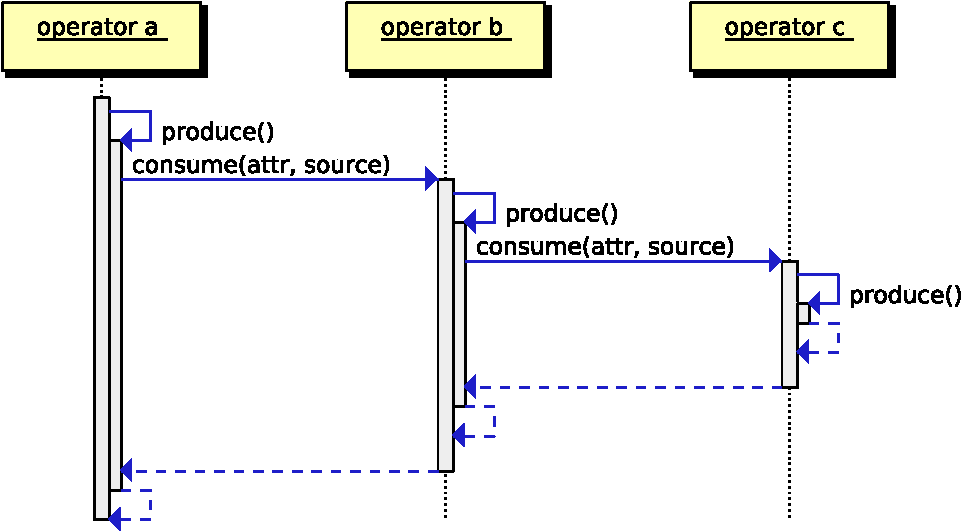
\includegraphics[scale=0.6]{figures/consume_produce}
  \caption[Consume Produce Sequence Diagram]{Consume Produce Sequence Diagram.}\label{fig:consume_produce_sd}
\end{figure}


Therefore, this programming model pushes data towards the next operator, instead of pulling the data. This results in a much better code and data locality. Tuples are pushed from one operator to the next, therefore operators benefit from keeping the data in the CPU registers, which allows very cheap and efficient computation. Thus, most computation is done using the CPU registers, only when materializing data memory has to be accessed. Additionally, small code fragments are used to handle large amounts of data in tight loops leading to good code locality and therefore high performance.
\\
Therefore, computation is very fast. However, what happens when data has to be materialized? Whenever we talk about taking tuples out of the CPU registers, i.e. materializing tuples in main memory, the operator pipeline breaks, therefore we call it a pipeline breaker. Materializes an operator all incoming tuples before continuing processing, we call it a full pipeline breaker. An example is a join operator: One side of the join relations has to be materialized in main memory,  while the other relation can be scanned and probe the materialized data for join partners. As the join operator takes data out of the registers we call it a pipeline breaker.
\\
It is important to note that the \texttt{consume produce} functions are just an abstraction layer for the programmer. This abstraction layer is used by the code generation to compile assembly code. Within the assembly code there is not \texttt{consume produce} present anymore.

\subsection{LLVM Code Compilation}

After an understanding of the HyPer operator programming model, next we discuss the query compilation in further detail. As in traditional systems, queries are compiled by parsing the query, translated into algebra and optimized. In contrast to a traditional system, the algebra is now not translated into physical algebra and executed, but compiled by the code generation into an imperative program. For this imperative program the \texttt{consume produce} model is used.
\\
For compiling the algebraic expressions into machine code, the first approach was to generate C++ code and load the result as a shared library at runtime. This seems logical because HyPer is already written in C++ and the shared library could access the existing data structures of the database system easily. On the other hand, compiling optimized C++ code is very slow and the compilation time can already take several seconds for a complex query, which is too slow for a database system. Additionally, the C++ compiler does not offer total control over the generated code, e.g. overflow flags are not available. 
\\
Therefore, queries are compiled into native machine code using the Low Level Virtual Machine (LLVM) compiler framework~\parencite{LLVM}. LLVM can generate portable assembler code which can be executed directly using an optimizing JIT compiler. With LLVM HyPer uses a very robust assembly code generation, e.g. pitfalls like register allocation are hidden by LLVM. Therefore the assembly code generation is very convenient compared to other compiler frameworks. Furthermore, only the LLVM JIT compiler translates the portable code into machine dependent code, leading to portable code across computer architectures. Since the LLVM assembler is strongly typed, many bugs can be caught in contrast to the original textual C++ code generation. Furthermore, LLVM produces highly optimized, extremely fast machine code and outperforms in some cases even hand-written code as the assembly language allows code optimization, hardware improvements and other tricks, that are hard to do in a high-level language as C++. All this requires usually only a few milliseconds of compilation time.
\\
Additionally, LLVM code is perfectly able to interact with C++, the main language of the HyPer database which is a big advantage. Even though LLVM code is robust and convenient to write compared to common assembler code, it is still more painful than writing code in a high-level language like C++. This enables us to implement the operators using both C++ and LLVM code, and reuse database logic such as index structures, that are already implemented in C++. 
\\
Therefore complex data structures or algorithms can be written in C++ and connected together by LLVM Code, where the C++ code is pre-compiled and the LLVM Code is compiled at runtime dynamically. This results also in a low query compilation time. An example is the Sort operator: The \texttt{compare} function, comparing two tuples by the rules of the sort query is dynamically generated in LLVM code, depending on the schema of the database. As actual sort function, the built-in C++ texttt{sort} can be used. This is a great example of the mixed execution model using both C++ and LLVM Code.
\\
Even though C++ and LLVM can both be used implementing an operator, LLVM code is dominant and C++ code should be seen as convenience. For performance gains, it is important that the code that is executed for most of the tuples is pure LLVM code, even though calling C++ from time to time is acceptable. As already mentioned, staying in LLVM allows us to keep the data in the CPU registers and is therefore the preferable way of executing a query. Calling an external function spills all registers to memory, which can be a bottleneck when doing this a million times, which is quite likely when using big amounts of data.
\\
As conclusion, we have shown that the HyPer programming model for operators implements a \texttt{consume produce} model to push data towards the next operator. Furthermore, the LLVM compiler framework is used for code generation and can be combined with C++ code at runtime. 
This division between LLVM and C++ code regarding programmer friendliness and execution time is one of the dominant patterns of the following sections.


\section{Requirements and Constraints}
Before we look at the technical implementation details in greater details, we discuss the requirements and constraints of our k-Means operator.
\\
Obviously, the k-Means algorithm must be implemented as a HyPer operator. That means, the \texttt{consume produce} programming model and the code generation with C++ and LLVM have to be used. The advantage of implementing k-Means as an operator is that it can be used in combination with other operators useful for data mining, such as grouping and aggregation functionalities.
\\
Regarding the functional aspects, the operator must be able to be executed in serial and in parallel, to make use of the computing power of modern workstations.
\\
As input parameters, the user can specify the number of maximum iterations of the algorithm. If this parameter is omitted, the algorithm runs until convergence. For big data sets this is often a performance problem when only a few data points are changing but all the distances have to be computed again. Often the result is already accurate enough after a specific number of iterations. Apart from an advantage regarding the running time it is also useful to specify the number of iterations for proper testing.
\\
Further parameters are the initialization strategy and a verbose option. As initialization strategy, the user can select between random initialization and the k-Means++ initialization. The verbose option let the algorithm to compute and to print additional information about the k-Means algorithm.
\\
As default output, an additional column is added to each data row presenting the cluster identifier of the data tuple as an integer. If the verbose option is active, statistics about the run are printed to the console. This information contains the number of iterations, the final center coordinates, the number of assigned data points per center and the squared error sum. 
\\
The number of iterations is  important for comparing the running time of different k-Means algorithms in a fair manner. It is possible that one run converges after three iterations, while another one converges after seven iterations. The number of iterations is non-deterministic since we are using a random initialization strategy. For fair evaluation, the time per iterations is therefore a good quality measurement.


\section{Data Materialization}

In this section we discuss the data materialization for the k-Means operator. As already stated, materialization is the process where we take our incoming tuples out of the CPU registers and write them into memory. Since this decreases the performance of the database, HyPer tries to avoid this process whenever possible and keeping the data in the pipeline until a pipeline breaker occurs. Unfortunately, k-Means is a pipeline breaker: E.g., center tuples have to be compared with all the data tuples to find the minimum distance between them. Therefore, we have to put all the incoming tuples in memory. That means, when the predecessing operator calls the \texttt{consume} function of the k-Means operator, each incoming tuple will be written into main memory, as ~\autoref{fig:mat1} shows. 

\begin{figure}[htsb]
  \centering
  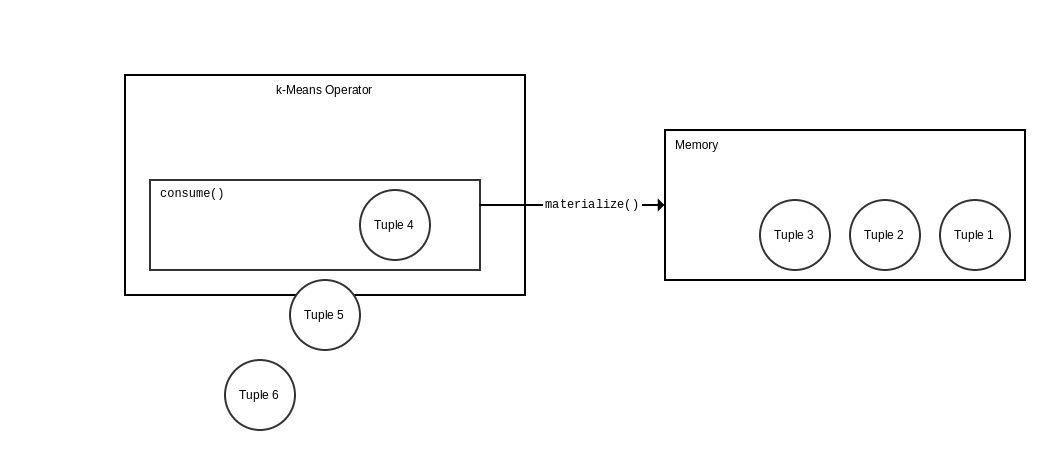
\includegraphics[scale=0.4]{figures/mat1}
  \caption[Data Materialization of Incoming Tuples]{Data Materialization of Incoming Tuples.}
  \label{fig:mat1}
\end{figure}

This is implemented by using a combination of LLVM and C++ code. In HyPer, LLVM Code resides in the \texttt{compile time system (cts)} while C++ resides in the \texttt{runtime system (rts)}. Since the \texttt{compile time system} is the entry point of an operator, the \texttt{consume} function is called and generates code for each tuple. This code is materializing the incoming tuples. A pointer to the materialized chunk of memory is then stored in a C++ vector in the \texttt{runtime system}. ~\autoref{fig:mat2} shows this process: Each tuple is materialized into memory by the \texttt{cts} and can be referenced by a pointer stored in a vector in the \texttt{rts}. This vector can later be used to loop through the entire data set: First by looping through the vector in C++, getting the pointers to the memory locations, which allows to load the tuple from memory and back to the CPU registers in the \texttt{cts}. 


\begin{figure}[htsb]
  \centering
  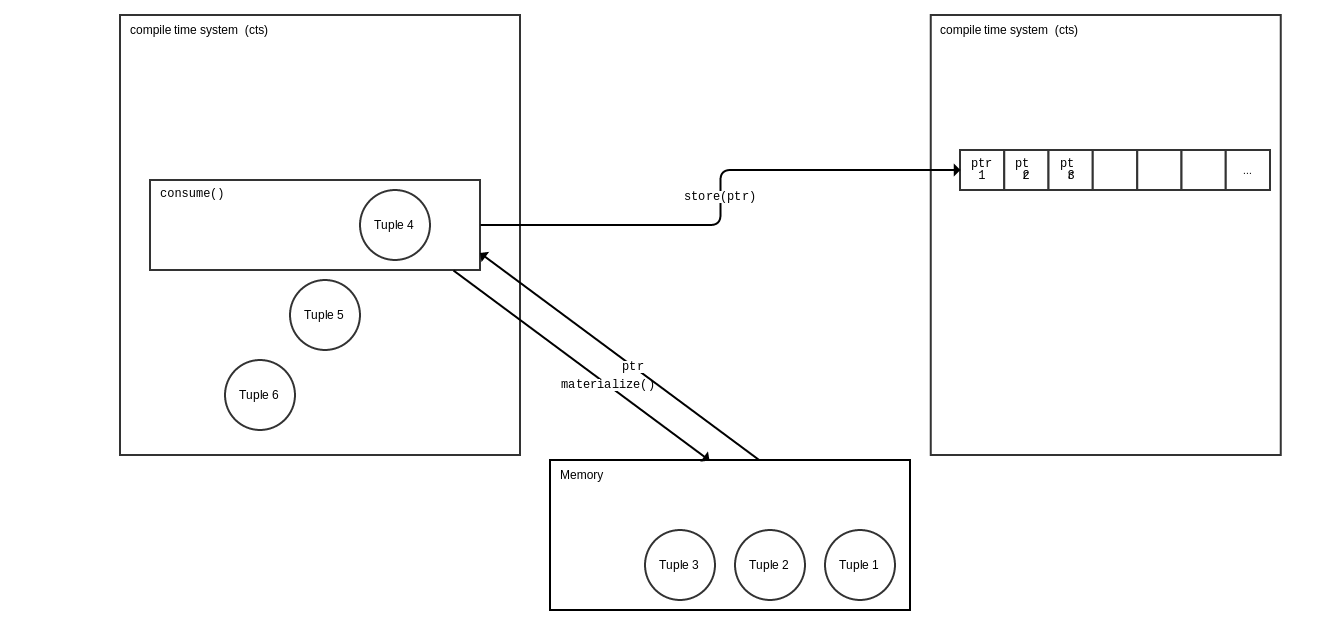
\includegraphics[scale=0.25]{figures/mat2}
  \caption[Data Materialization using the Runtime and Compile Time System]{Data Materialization using the Runtime and Compile Time System.}
  \label{fig:mat2}
\end{figure}

For k-Means it is not enough to store only the data tuples. We also need to reserve memory space for the centers. We do this by materializing the first \texttt{k} tuples of the data set two times: Once as storage for data tuples and once as storage for center tuples. Therefore we have two vectors in the \texttt{runtime system}: One for data tuples of length \texttt{n}, and one for centers of length \texttt{k}. This data materialization for k-Means is depicted in ~\autoref{fig:mat3}.
\\ 
All data tuples and centers are materialized and an additional field has been added to all of them: A cluster identifier of type \texttt{integer}. For the center tuples, this field stores the center identifier, which is 0 to \texttt{k}. For data tuples, this field specifies to which center a data tuple belongs to. Initially, all data tuples are assigned to the center with identifier 0. 
\\
Another difference is the change of data types between data and center tuples. While the data types of data tuples are specified in the table schema, the data types of the center tuples are determined differently since the center is the mean of all the data tuples assigned to that center. Therefore, an \texttt{integer} data value is stored as a \texttt{Numeric} data type as center value. Hence, the mean of an integer can be stored in the center field. For each data type there exists a rule to converse the type from data tuple to center tuple.



\begin{figure}[htsb]
  \centering
  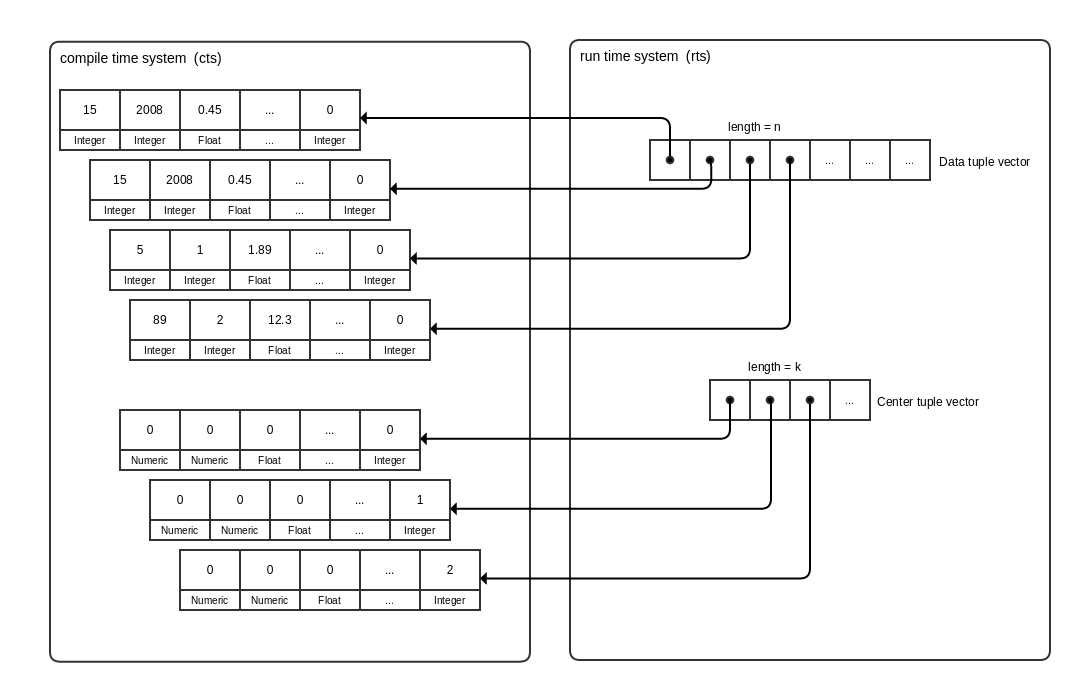
\includegraphics[scale=0.25]{figures/mat3}
  \caption[k-Means Data Materialization in Detail]{k-Means Data Materialization in Detail.}
  \label{fig:mat3}
\end{figure}




\section{Serial Implementation}

After acquiring a basic understanding of HyPer’s operator model, in particular about the interaction of dynamically generated LLVM code and pre-compiled C++ code, we can discuss the actual implementation of a serial k-Means algorithm. The most interesting part of implementing a data mining operator like k-Means is the decision about how to implement the algorithm, e.g. which parts should reside in the \texttt{compile time system} and which parts in the \texttt{run time system}. 
\\
This question is not trivial because there are no strict rules and several possibilities. A dynamic generation of code works best for comparing tuples with each other as in the sort operator, or the computation of a distance in the k-Means operator. This code has to handle different data types depending on the table schema and therefore LLVM code is preferable. For other parts, like the implementation of a sort function or the combination of loops in k-Means, it is not so obvious where to put the code.
\\
In this work we present two different ways of implementing a serial k-Means Operator in HyPer, first by implementing the algorithm in C++ and using only a few generated LLVM functions, e.g. to compute the distance. Secondly, a system is presented implementing k-Means almost entirely in LLVM. Only small parts, like initializing the random centers are implemented in C++.



\subsection{A C++ driven Implementation}

As first implementation approach we present a C++ driven version. The term C++ driven is maybe misleading, since all operators are doing their main computation after executing their \texttt{consume} function, which is a LLVM generated method. Even though the operator starts working in the \texttt{compile time system}, in this implementation, \texttt{cts} calls the k-Means operator of the \texttt{runtime system} and gives the full control to the C++ code, until the k-Means algorithm terminates. 

~\autoref{fig:cpp_driven} shows this interaction in a sequence diagram. The algorithm is invoked in the \texttt{compile time system} and calls the k-Means function of the \texttt{runtime system}. The entire execution stays now in the \text{runtime system}, with calls back to LLVM from time to time. 
\\
First, the centers are picked. Let’s assume we are using a random initialization strategy. \texttt{K} times, a random pointer of the data vector is selected, and its values are then written to the corresponding center tuple. Therefore, a \texttt{centerPtr} and a random \texttt{dataPtr} are parameters of a generated \texttt{setCenter} function. There, the data tuple and the center tuple are loaded from memory using the two pointers. Data values are casted if necessary, since we have different data types among center tuples and data tuples, and then stored in the center tuple. Afterwards, the center tuple is written back to memory.

\begin{figure}[htsb]
  \centering
  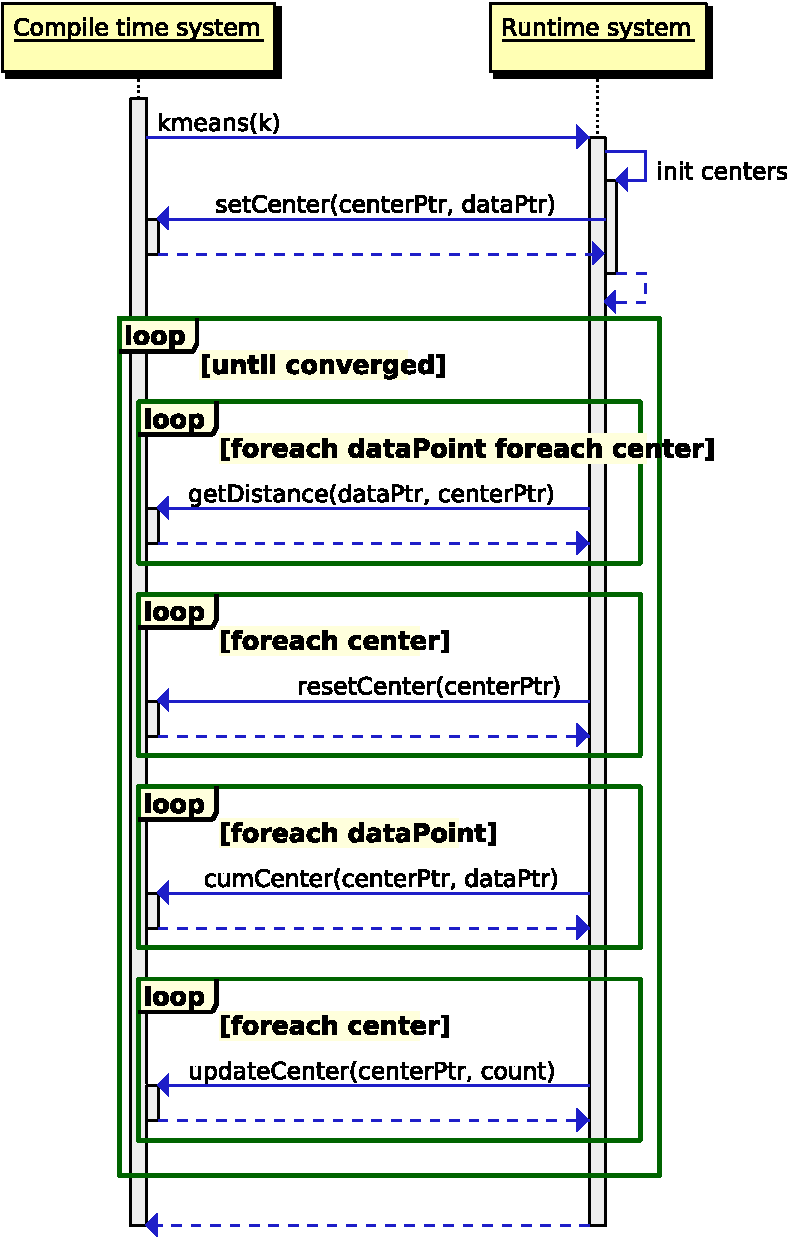
\includegraphics[scale=0.35]{figures/cpp_driven}
  \caption[The k-Means Algorithm - C++ driven]{The k-Means Algorithm - C++ driven.}
  \label{fig:cpp_driven}
\end{figure}

After selecting the initial set of centers, the \texttt{runtime system} starts its outer loop, running until k-Means converges. In the outer loop, the \texttt{runtime system} calls the \texttt{compile time system} to compute the distances between all data points and all center points to find the closest center for each data tuple. Therefore, \texttt{getDistance} is called for each \texttt{dataPtr} - \texttt{centerPtr} combination. The closest center for each data point is stored in a \texttt{unordered\_map} in C++. 
\\
After finding the closest center for each data tuple, the centers have to be updated. Since the materialization of centers is done in LLVM code, the \texttt{runtime system} has to call the \texttt{compile time system} again, in fact even several times: First, a \texttt{resetCenter} function is called for all center pointers to set the center values of the center tuples to zero. Then, the new mean can be computed. 
\\
This is done in two steps. First, the data points are accumulated for each center, and then divided by the number of data points belonging to each center. This simple mean computation leads to several \texttt{code time system} calls for our algorithm. For each data point, the values are added to the center tuple it belongs to. Therefore, the \texttt{cumCenter} function is called, adding the data point to the center point and also updates the cluster identifier of the data tuple. The \texttt{runtime system} keeps count about how many tuples are added to each center. When finished, each center is called again with this count to compute the actual mean of the center using the \texttt{updateCenter} function. This process continues until the algorithm converges.
\\
As we see, the main control of the algorithm remains in the \texttt{runtime system}. However, this kind of implementation leads to many calls between the \texttt{compile time} and the \texttt{runtime system}, in total $(n+2) \cdot k + n$ per iteration, as ~\autoref{tab:llvm_calls} shows. The next sections presents an implementation that prevents the algorithms from too many calls between the two systems.




\begin{table}[htsb]
  \caption[LLVM number of calls]{Generated Function's Calls per Iteration.}\label{tab:llvm_calls}
  \centering
  \begin{tabular}{l l}
    \toprule
      Generated Function & Calls per Iteration \\
    \midrule
      \texttt{getDistance} & $k \cdot n$ \\
      \texttt{resetCenter} & $k$ \\
      \texttt{cumCenter} & $n$ \\
      \texttt{updateCenter} & $k$ \\
    \bottomrule
      Total & $k \cdot n + k + n + k = (n + 2) \cdot k + n$ \\
  \end{tabular}
\end{table}


\subsection{A LLVM driven Implementation}

As already stated, LLVM code generation encourages the interaction between LLVM and C++ code which is exploited a lot in the C++ driven implementation of k-Means: The algorithm is implemented in C++ and benefits from high level data structures like \texttt{unordered\_maps} and the convenience of the C++ syntax, allowing a quick implementation. 
\\
However, this leads to many calls between the \texttt{compile time} and the \texttt{runtime system}, as shown in ~\autoref{tab:llvm_calls}, which could possibly affect the performance of the operator. Therefore, a second approach has been explored, implementing the k-Means algorithm almost entirely in LLVM code. Only the random initialization of the center points remains in C++. When thinking about such an implementation, we have to be aware that we cannot use C++ data structures any more, but have to work with what LLVM gives us.


\begin{figure}[htsb]
  \centering
  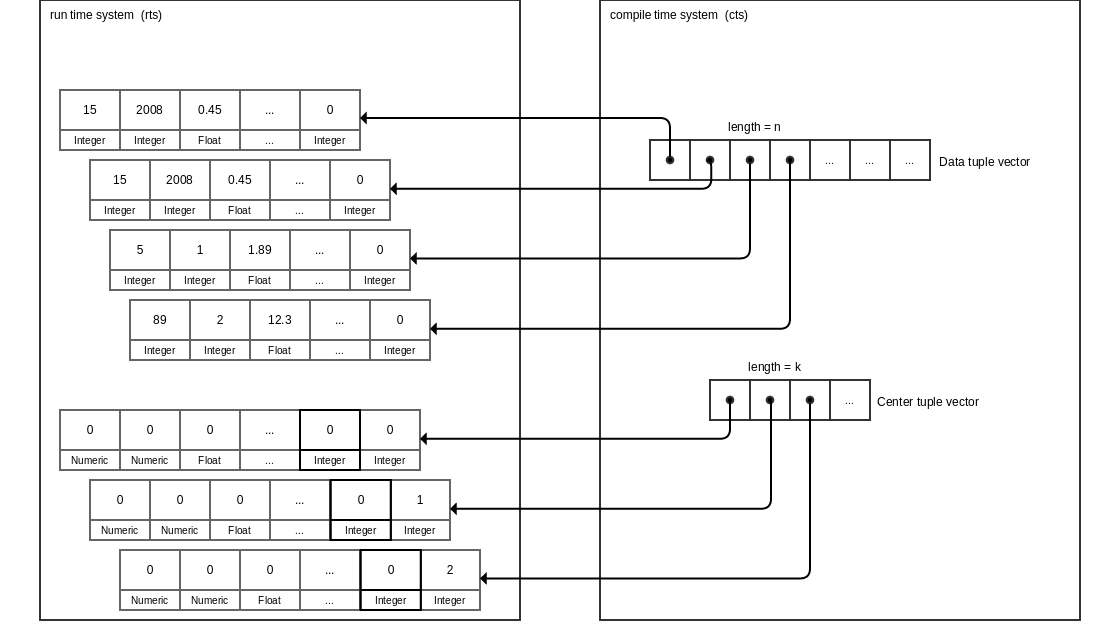
\includegraphics[scale=0.25]{figures/mat4}
  \caption[k-Means Data Materialization for the LLVM Implementation]{k-Means Data Materialization for the LLVM Implementation.}
  \label{fig:mat4}
\end{figure}

The only data structure we have used so far in LLVM was a structure to materialize the data and center tuples. In order to keep things simple, we exploit this data structure even further to use it with the LLVM k-Means implementation, without using any other data structures in addition.
So the question is how to extend the existing data structure of the \texttt{compile time system} to emulate the C++ code we want to omit? This is done by extending the center data structure when materializing the centers in the \texttt{consume} function. As ~\autoref{fig:mat4} shows, an additional field has been added to the center tuple, storing the count, i.e. how many data points are close to this center. With this small modification we can implement our algorithm in LLVM with the use of only one data structure.
\\
The algorithm is depicted in a sequence diagram in ~\autoref{fig:llvm_driven} and shows the indirection of the calls compared to the sequence diagram in ~\autoref{fig:cpp_driven}: This time, the LLVM code executes the algorithms, calling C++ code from time to time. There are also no loops around the calls between the LLVM and C++ code, therefore the number of calls is very low. 
\\
The initial center setting process does not change, but after this the control of the code goes back to the~\texttt{compile time system}. The only thing the~\texttt{compile time system} requires from the~\texttt{runtime system} are the first pointers and the last pointers of the data vector and of the center vector, respectively. Then, the~\texttt{compile time system} is ready to execute the k-Means algorithm without any further interaction with the~\texttt{runtime system}. 
\\
First, the minimum distances are computed between center and data tuples. The distance function was already implemented in LLVM code for the C++ driven approach and can be reused, only the loops around the \texttt{getDistance} function have to be implemented in LLVM. 
\\
The next step is to update the center tuples. The \texttt{resetCenter} function can be kept the same, as well as the \text{cumCenter} function. Again, the loops around are now implemented in pure LLVM code. When computing the mean of a center, we have to keep track of the count. For that purpose we are using the additional field each center tuple gets on data materialization. When adding data tuples to the corresponding center, we increment the count. At the end, when invoking the \texttt{updateCenter} function, this count is used to compute the mean. 



\begin{figure}[htsb]
  \centering
  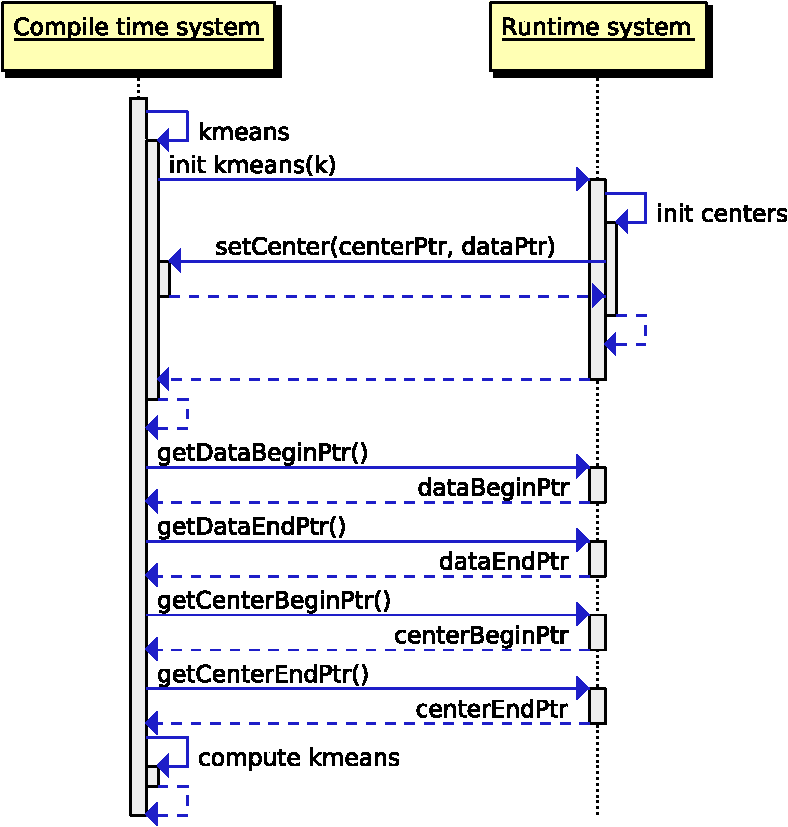
\includegraphics[scale=0.4]{figures/llvm_driven}
  \caption[The k-Means Algorithm - LLVM driven]{The k-Means Algorithm - LLVM driven.}
  \label{fig:llvm_driven}
\end{figure}



Even though the differences between the two presented approaches do not seem to be huge, since the overall programming concept remains the same, the difference in the code is significant. In particular using LLVM over high-level C++ constructs adds an overhead in the number of code lines. Therefore, the LLVM code in the second approach is harder to understand and to maintain. On the other hand, we are shrinking the number of calls between the C++ and LLVM system from $(n + 2) \cdot k + n$ down to 4. An evaluation chapter will show how this affects the performance of the two serial implementations.


\subsection{Initialization strategy}

So far we discussed the implementation details of our k-Means algorithm without paying attention to the used initialization strategy. As shown in chapter \ref{chapter:kmeans}, kmeans uses a random initialization strategy by default. A random initialzation strategy is easy to implement in the \texttt{runtime system}, since only C++ code is used finding a random subset of length \texttt{k} of the data tuples. This can be implemented using the Fisher-Yates shuffle algorithm~\parencite{fisheryates}. 
\\
When discussing k-Means we figured out that one of the most popular variations of k-Means is k-Means++. The k-Means++ algorithm uses an extended initialization strategy by choosing data points as center with higher probability the further away they are from the already chosen set of center points. Often, this leads to improvements in both speed and accuracy of the clustering.
\\
For implementation we have to compute the distance from the chosen center points to the data points already in the initialization phase. This can be done very conveniently for the C++ version, as the \texttt{getDistance} function is implemented already. Therefore, the main initialization routine can be written in C++, only the \texttt{getDistance} function is used as generated function.
\\
For the LLVM version, we still keep the center initialzation in the \texttt{runtime system} to benefit of high level C++ program structures. To execute the k-Means++ algorithm, we have to add a explicitly generated \texttt{getDistance} function to the LLVM code: Even though the LLVM version computes the distance as well, there is no generated function anymore, since the function is just part of LLVM code. Once we have added this function, k-Means++ can be implemented the same way as in the C++ driven approach.

\section{Parallel k-Means}

After looking at single-threaded implementations of the k-Means algorithm, in this section we show an approach to implement k-Means in HyPer in a parallel way to make use of all cores. Keeping in mind that HyPer is a high-performance database system written in C++, it makes already excessive use of multi-threaded programs, therefore it is only logical to add a parallel version of k-Means too. In the following we use the serial C++ version and modify it to allow parallelism. The C++ version is used over the LLVM version because of higher maintainability and readability. 
\\
The main bottleneck of the serial implementation is to compute the closest center for each data point: For each data point we have to calculate the distance to each center point which has to be done in each iteration. This means $k \cdot n$ distance computations, which can benefit a lot from parallelism.
\\
When executing a HyPer operator in parallel, the consume function is called for chunks of input tuples instead of the entire data set. Consider a system with four threads as shown in~\autoref{fig:parallel}: Each thread consumes one fourth of the data set and materializes the input tuples. In the runtime system, there are vectors for each thread, storing the pointers to the input tuples. 


\begin{figure}[htsb]
  \centering
  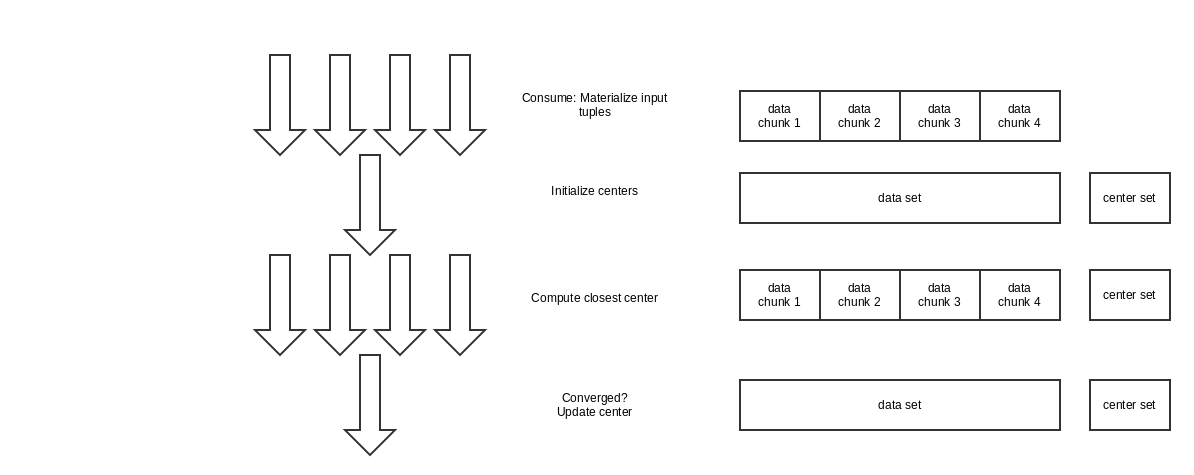
\includegraphics[scale=0.3]{figures/parallel}
  \caption[The k-Means Algorithm as Parallel Operator]{The k-Means Algorithm as Parallel Operator.}
  \label{fig:parallel}
\end{figure}

After consuming the data the k-Means algorithm continues with finding the initial center set. For that, we have to break the parallelism. For random initialization of the clusters, center tuples are selected from the entire data set. This is even more important for the k-Means++ initialization strategy computing centers regarding a distance function. While we could select random data points for the the center just from one data chunk, this is not possible for the k-Means++ initialization strategy anymore. Therefore, we create a global vector storing pointers to all materialization tuples. Now we can select the global center points by one of our initialization strategies and continue the parallel program sequence afterwards.
\\
After the serial initialization we jump back to parallel execution: The algorithm computes the distance from each data point to each center point. For each data chunk we compute the distances on a separate thread. With omitting the overhead for process creation and management, this could lead to a running time advantage of one fourth of the serial execution.
\\
Afterwards, we jump back to a serial execution of the program and check for each thread if the program converged. Only if all threads converged, we can terminate the algorithm and output the result of the clustering. Otherwise, we update the global centers by the newly assigned data points. In the first version of this implementation, this step is done in serial, but here is also potential to parallelize the program.
\\
In the evaluation chapter we compare the parallel k-Means algorithm with the serial implementations. Even though only one part of the algorithm is parallelized and with the overhead of by introducing the parallelism, we expect huge performance gains.





